% Options for packages loaded elsewhere
\PassOptionsToPackage{unicode}{hyperref}
\PassOptionsToPackage{hyphens}{url}
%
\documentclass[
]{article}
\usepackage{amsmath,amssymb}
\usepackage{iftex}
\ifPDFTeX
  \usepackage[T1]{fontenc}
  \usepackage[utf8]{inputenc}
  \usepackage{textcomp} % provide euro and other symbols
\else % if luatex or xetex
  \usepackage{unicode-math} % this also loads fontspec
  \defaultfontfeatures{Scale=MatchLowercase}
  \defaultfontfeatures[\rmfamily]{Ligatures=TeX,Scale=1}
\fi
\usepackage{lmodern}
\ifPDFTeX\else
  % xetex/luatex font selection
\fi
% Use upquote if available, for straight quotes in verbatim environments
\IfFileExists{upquote.sty}{\usepackage{upquote}}{}
\IfFileExists{microtype.sty}{% use microtype if available
  \usepackage[]{microtype}
  \UseMicrotypeSet[protrusion]{basicmath} % disable protrusion for tt fonts
}{}
\makeatletter
\@ifundefined{KOMAClassName}{% if non-KOMA class
  \IfFileExists{parskip.sty}{%
    \usepackage{parskip}
  }{% else
    \setlength{\parindent}{0pt}
    \setlength{\parskip}{6pt plus 2pt minus 1pt}}
}{% if KOMA class
  \KOMAoptions{parskip=half}}
\makeatother
\usepackage{xcolor}
\usepackage[margin=1in]{geometry}
\usepackage{graphicx}
\makeatletter
\def\maxwidth{\ifdim\Gin@nat@width>\linewidth\linewidth\else\Gin@nat@width\fi}
\def\maxheight{\ifdim\Gin@nat@height>\textheight\textheight\else\Gin@nat@height\fi}
\makeatother
% Scale images if necessary, so that they will not overflow the page
% margins by default, and it is still possible to overwrite the defaults
% using explicit options in \includegraphics[width, height, ...]{}
\setkeys{Gin}{width=\maxwidth,height=\maxheight,keepaspectratio}
% Set default figure placement to htbp
\makeatletter
\def\fps@figure{htbp}
\makeatother
\setlength{\emergencystretch}{3em} % prevent overfull lines
\providecommand{\tightlist}{%
  \setlength{\itemsep}{0pt}\setlength{\parskip}{0pt}}
\setcounter{secnumdepth}{-\maxdimen} % remove section numbering
\usepackage{tikz}
\usepackage{pgfplots}
\pgfplotsset{compat=1.18}
\usetikzlibrary{shapes, positioning, calc, decorations.markings, chains, scopes}
\newlength{\Radius}
\setlength\Radius{4em}
\usepackage{amsmath}
\usepackage{caption}
\ifLuaTeX
  \usepackage{selnolig}  % disable illegal ligatures
\fi
\IfFileExists{bookmark.sty}{\usepackage{bookmark}}{\usepackage{hyperref}}
\IfFileExists{xurl.sty}{\usepackage{xurl}}{} % add URL line breaks if available
\urlstyle{same}
\hypersetup{
  hidelinks,
  pdfcreator={LaTeX via pandoc}}

\author{}
\date{\vspace{-2.5em}}

\begin{document}

\begin{figure}
\centering
\caption*{Decomposition.}
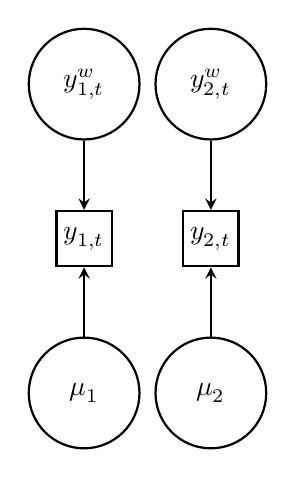
\begin{tikzpicture}[
    auto, > = latex, align=center,
    latent/.style = {
      circle, draw, thick, inner sep = 2pt, minimum width = \Radius
    },
    manifest/.style = {
      rectangle, draw, thick, inner sep = 0pt, minimum size = \Radius/2
    },
    intercept/.style = {
      regular polygon,regular polygon sides = 3, draw, thick,
      inner sep = 0pt, minimum size = \Radius
    },
    mean/.style = {
      regular polygon, regular polygon sides = 3, draw, thick,
      inner sep = 0pt, minimum size = 8mm
    },
    path/.style = {
      arrows = ->, thick, > = {stealth[]}
    },
    error/.style = {
      circle, draw = none, fill = none, thick,
      inner sep = 0pt, minimum size = 5mm
    },
    var/.style = {
      <->, thick, > = {stealth[]}, bend right = 270, looseness = 2
    },
    cov/.style = {
      <->, thick, > = {stealth[]}, bend right = 300
    },
    % style to add a circle in the middle of a path
    random/.style = {
      postaction = {
        decorate, decoration = {
          markings,
          mark = at position .5 with {
            \draw[fill = black] circle[radius = 2pt];
          }
        }
      }
    },
    random_cl/.style = {
      postaction = {decorate, decoration = {
        markings,
        mark = at position .2 with {
          \draw[fill = black] circle[radius = 2pt];}
        }
      }
    },
    ]

    % draw decomposition
    \node  [manifest]  (y1t)  {$y_{1,t}$};
    \node  [latent]  (y1wt)  [above = 2.5em of y1t]  {$y_{1,t}^w$};
    \node  [latent]  (mu_1)  [below = 2.5em of y1t]  {$\mu_{1}$};

    % draw nodes
    \foreach \i [remember = \i as \lasti (initially 1)] in {2, ..., 2}
    \node  [manifest]  (y\i t)  [right = 2.5em of y\lasti t]  {$y_{\i,t}$};

    \foreach \i [remember = \i as \lasti (initially 1)] in {2, ..., 2}
    \node  [latent]  (y\i wt)  [above = 2.5em of y\i t]  {$y_{\i,t}^w$};

    \foreach \i [remember = \i as \lasti (initially 1)] in {2, ...,2}
    \node  [latent]  (mu_\i)  [below = 2.5em of y\i t]  {$\mu_{\i}$};

    % draw paths
    \foreach \i [remember = \i as \lasti (initially 1)] in {1, ...,2}
    \draw  [path]  (y\i wt)  to node  []  {}  (y\i t);

    \foreach \i [remember = \i as \lasti (initially 1)] in {1, ...,2}
    \draw  [path]  (mu_\i)  to node  []  {}  (y\i t);
    
\end{tikzpicture}
\end{figure}

\begin{figure}
\centering
\caption*{Within-model.}
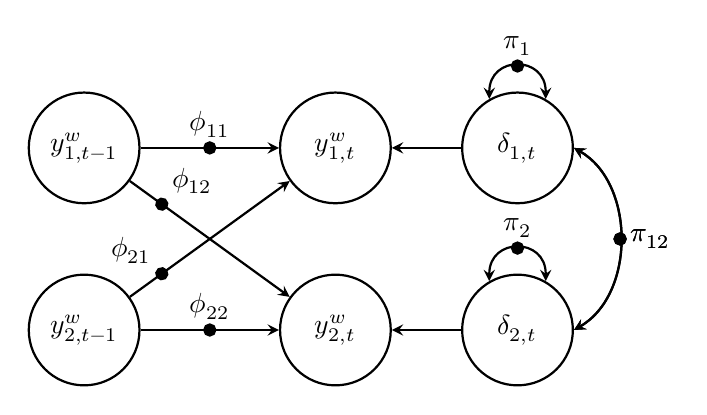
\begin{tikzpicture}[
    auto, > = latex, align=center,
    latent/.style = {
      circle, draw, thick, inner sep = 2pt, minimum width = \Radius
    },
    manifest/.style = {
      rectangle, draw, thick, inner sep = 0pt, minimum size = \Radius/2
    },
    intercept/.style = {
      regular polygon,regular polygon sides = 3, draw, thick,
      inner sep = 0pt, minimum size = \Radius
    },
    mean/.style = {
      regular polygon, regular polygon sides = 3, draw, thick,
      inner sep = 0pt, minimum size = 8mm
    },
    path/.style = {
      arrows = ->, thick, > = {stealth[]}
    },
    error/.style = {
      circle, draw = none, fill = none, thick,
      inner sep = 0pt, minimum size = 5mm
    },
    var/.style = {
      <->, thick, > = {stealth[]}, bend right = 270, looseness = 2
    },
    cov/.style = {
      <->, thick, > = {stealth[]}, bend right = 300
    },
    % style to add a circle in the middle of a path
    random/.style = {
      postaction = {
        decorate, decoration = {
          markings,
          mark = at position .5 with {
            \draw[fill = black] circle[radius = 2pt];
          }
        }
      }
    },
    random_cl/.style = {
      postaction = {decorate, decoration = {
        markings,
        mark = at position .2 with {
          \draw[fill = black] circle[radius = 2pt];}
        }
      }
    },
    ]

    % draw within-level structural model
    \node  [latent]  (y1wt-1)  {$y_{1,t-1}^w$};
    \node  [latent]  (y1wt)  [right =5em of y1wt-1]  {$y_{1,t}^w$};
    \node  [latent]  (delta1t)  [right =2.5em of y1wt]  {$\delta_{1,t}$};

    % draw nodes
    \foreach \i [remember = \i as \lasti (initially 1)] in {2, ..., 2}
    \node  [latent]  (y\i wt-1)  [below = 2.5em of y\lasti wt-1]  {$y_{\i ,t-1}^w$};

    \foreach \i [remember = \i as \lasti (initially 1)] in {2, ..., 2}
    \node  [latent]  (y\i wt)  [below = 2.5em of y\lasti wt]  {$y_{\i ,t}^w$};

    \foreach \i [remember = \i as \lasti (initially 1)] in {2, ..., 2}
    \node  [latent]  (delta\i t)  [below = 2.5em of delta\lasti t]  {$\delta_{\i ,t}$};

    % draw paths from residuals to yiwt
    \foreach \i [remember = \i as \lasti (initially 1)] in {1, ...,2}
    \draw  [path]  (delta\i t)  to node  []  {}  (y\i wt);
    
\draw  [path, postaction = random]  (y1wt-1)  to node  []  {$\phi_{11}$}  (y1wt);
\draw  [path, postaction = random_cl]  (y1wt-1)  to node  [pos = .2]  {$\phi_{12}$}  (y2wt);
\draw  [path, postaction = random_cl]  (y2wt-1)  to node  [pos = .2]  {$\phi_{21}$}  (y1wt);
\draw  [path, postaction = random]  (y2wt-1)  to node  []  {$\phi_{22}$}  (y2wt);

\draw  [var, postaction = random]  (delta1t.120)  to node  []  {$\pi_{1}$}  (delta1t.60);
 \draw  [cov, postaction = random]  (delta1t.0)  to node  []  {$\pi_{12}$}  (delta2t.0);
\draw  [var, postaction = random]  (delta2t.120)  to node  []  {$\pi_{2}$}  (delta2t.60);
 \draw  [cov, postaction = random]  (delta1t.0)  to node  []  {$\pi_{12}$}  (delta2t.0);

\end{tikzpicture}
\end{figure}

\begin{figure}
\centering
\caption*{Between-model.}
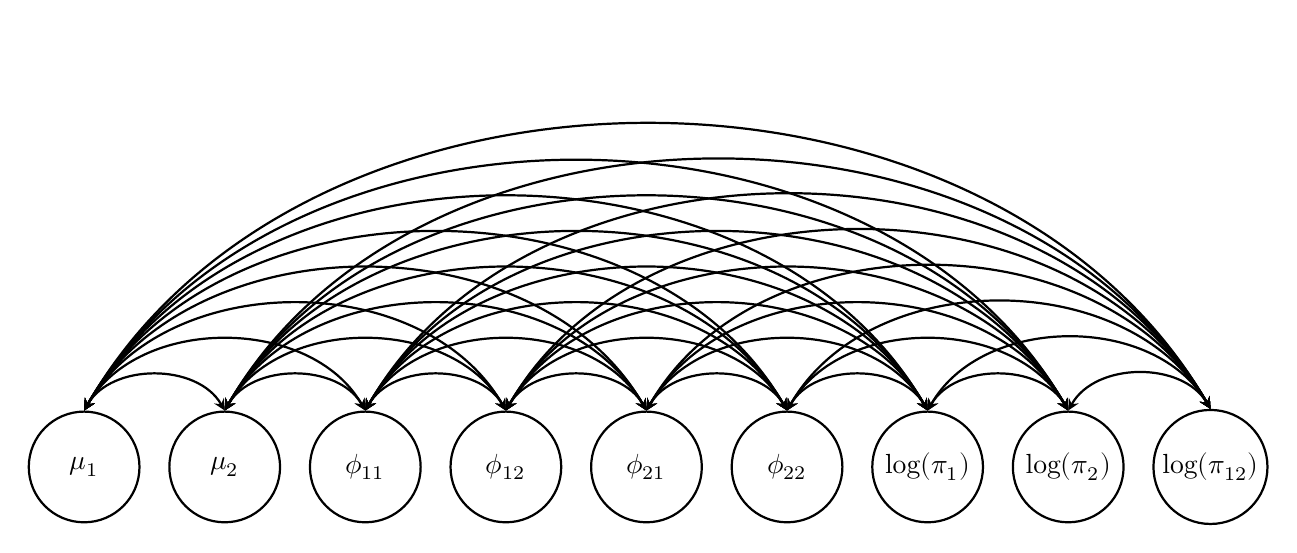
\begin{tikzpicture}[
    auto, > = latex, align=center,
    latent/.style = {
      circle, draw, thick, inner sep = 2pt, minimum width = \Radius
    },
    manifest/.style = {
      rectangle, draw, thick, inner sep = 0pt, minimum size = \Radius/2
    },
    intercept/.style = {
      regular polygon,regular polygon sides = 3, draw, thick,
      inner sep = 0pt, minimum size = \Radius
    },
    mean/.style = {
      regular polygon, regular polygon sides = 3, draw, thick,
      inner sep = 0pt, minimum size = 8mm
    },
    path/.style = {
      arrows = ->, thick, > = {stealth[]}
    },
    error/.style = {
      circle, draw = none, fill = none, thick,
      inner sep = 0pt, minimum size = 5mm
    },
    var/.style = {
      <->, thick, > = {stealth[]}, bend right = 270, looseness = 2
    },
    cov/.style = {
      <->, thick, > = {stealth[]}, bend right = 300
    },
    % style to add a circle in the middle of a path
    random/.style = {
      postaction = {
        decorate, decoration = {
          markings,
          mark = at position .5 with {
            \draw[fill = black] circle[radius = 2pt];
          }
        }
      }
    },
    random_cl/.style = {
      postaction = {decorate, decoration = {
        markings,
        mark = at position .2 with {
          \draw[fill = black] circle[radius = 2pt];}
        }
      }
    },
    ]
\node  [latent]  (mu_1)  {$\mu_{1}$};
\node  [latent]  (mu_2)  [right = 1em of mu_1]  {$\mu_{2}$};
\node  [latent]  (phi_11)  [right = 1em of mu_2]  {$\phi_{11}$};
\node  [latent]  (phi_12)  [right = 1em of phi_11]  {$\phi_{12}$};
\node  [latent]  (phi_21)  [right = 1em of phi_12]  {$\phi_{21}$};
\node  [latent]  (phi_22)  [right = 1em of phi_21]  {$\phi_{22}$};
\node  [latent]  (lnsigma2_1)  [right = 1em of phi_22]  {$\log(\pi_{1})$};
\node  [latent]  (lnsigma2_2)  [right = 1em of lnsigma2_1]  {$\log(\pi_{2})$};
\node  [latent]  (lnsigma_12)  [right = 1em of lnsigma2_2]  {$\log(\pi_{12})$};

\draw  [cov]  (mu_1.north)  to node  []  {}  (mu_2.north);
\draw  [cov]  (mu_1.north)  to node  []  {}  (phi_11.north);
\draw  [cov]  (mu_1.north)  to node  []  {}  (phi_12.north);
\draw  [cov]  (mu_1.north)  to node  []  {}  (phi_21.north);
\draw  [cov]  (mu_1.north)  to node  []  {}  (phi_22.north);
\draw  [cov]  (mu_1.north)  to node  []  {}  (lnsigma2_1.north);
\draw  [cov]  (mu_1.north)  to node  []  {}  (lnsigma2_2.north);
\draw  [cov]  (mu_1.north)  to node  []  {}  (lnsigma_12.north);
\draw  [cov]  (mu_2.north)  to node  []  {}  (phi_11.north);
\draw  [cov]  (mu_2.north)  to node  []  {}  (phi_12.north);
\draw  [cov]  (mu_2.north)  to node  []  {}  (phi_21.north);
\draw  [cov]  (mu_2.north)  to node  []  {}  (phi_22.north);
\draw  [cov]  (mu_2.north)  to node  []  {}  (lnsigma2_1.north);
\draw  [cov]  (mu_2.north)  to node  []  {}  (lnsigma2_2.north);
\draw  [cov]  (mu_2.north)  to node  []  {}  (lnsigma_12.north);
\draw  [cov]  (phi_11.north)  to node  []  {}  (phi_12.north);
\draw  [cov]  (phi_11.north)  to node  []  {}  (phi_21.north);
\draw  [cov]  (phi_11.north)  to node  []  {}  (phi_22.north);
\draw  [cov]  (phi_11.north)  to node  []  {}  (lnsigma2_1.north);
\draw  [cov]  (phi_11.north)  to node  []  {}  (lnsigma2_2.north);
\draw  [cov]  (phi_11.north)  to node  []  {}  (lnsigma_12.north);
\draw  [cov]  (phi_12.north)  to node  []  {}  (phi_21.north);
\draw  [cov]  (phi_12.north)  to node  []  {}  (phi_22.north);
\draw  [cov]  (phi_12.north)  to node  []  {}  (lnsigma2_1.north);
\draw  [cov]  (phi_12.north)  to node  []  {}  (lnsigma2_2.north);
\draw  [cov]  (phi_12.north)  to node  []  {}  (lnsigma_12.north);
\draw  [cov]  (phi_21.north)  to node  []  {}  (phi_22.north);
\draw  [cov]  (phi_21.north)  to node  []  {}  (lnsigma2_1.north);
\draw  [cov]  (phi_21.north)  to node  []  {}  (lnsigma2_2.north);
\draw  [cov]  (phi_21.north)  to node  []  {}  (lnsigma_12.north);
\draw  [cov]  (phi_22.north)  to node  []  {}  (lnsigma2_1.north);
\draw  [cov]  (phi_22.north)  to node  []  {}  (lnsigma2_2.north);
\draw  [cov]  (phi_22.north)  to node  []  {}  (lnsigma_12.north);
\draw  [cov]  (lnsigma2_1.north)  to node  []  {}  (lnsigma2_2.north);
\draw  [cov]  (lnsigma2_1.north)  to node  []  {}  (lnsigma_12.north);
\draw  [cov]  (lnsigma2_2.north)  to node  []  {}  (lnsigma_12.north);

\end{tikzpicture}
\end{figure}

\end{document}
